\documentclass{beamer}
\usepackage{graphicx}
\usepackage[spanish]{babel} % para escribir en espanol
\usepackage[utf8]{inputenc}

\usetheme{Madrid}

\title{Tu ciudad}
\subtitle{Metodologías de Desarrollo Ágil}

\author{David Infante Casas \and Laura Gómez Garrido \and Pedro Bonilla Nadal \and Juan Ocaña Valenzuela \and Antonio Martín Ruíz }

\AtBeginSection[]
{
  \begin{frame}<beamer>{}
    \tableofcontents[currentsection,currentsubsection]
  \end{frame}
}

\begin{document}
\begin{frame}
\titlepage
\end{frame}
\begin{frame}{Contenido}
  \tableofcontents
  % You might wish to add the option [pausesections]
\end{frame}
\section{División de tareas y
asignación}
\subsection{Primer Sprint}

\begin{frame}{Primer Sprint}
\begin{table}[]
\resizebox{10cm}{!}{
\begin{tabular}{|l|l|l|}
\hline
\multicolumn{1}{|c|}{\textbf{Tarea}} & \multicolumn{1}{|c|}{\textbf{Historias Usuario}} & \multicolumn{1}{|c|}{\textbf{Asignado }}\\ \hline
Diseño BD & HU1 HU8 & Laura\\ \hline
Conexión con API mapas & HU1 & Antonio\\ \hline
Conexión con BD & HU1 & Laura\\ \hline
Diseño GUI & HU1 & Juan\\ \hline
Implementación GUI & HU1 & David\\ \hline
Conexión front-end/back-end & HU1 & Pedro\\ \hline
Botón de mapa & HU8 HU9 HU3 HU4 & Juan\\ \hline
Botón de información & HU8 & Pedro\\ \hline
Menú de lista & HU8 & Antonio\\ \hline
Diseño de clase base & HU9 HU3 HU4 & David\\ \hline
Interfaz de información & HU9 HU3 HU4 & Laura\\ \hline
Clase contenedor & HU9 & Pedro\\ \hline
Clase fuente & HU3 & Antonio\\ \hline
Clase parque & HU4 & Juan\\ \hline
\end{tabular}
}
\end{table}

\end{frame}

\subsection{Segundo Sprint}

\begin{frame}{Segundo Sprint}

\begin{table}[]
\resizebox{9.5cm}{!}{
\begin{tabular}{|l|l|l|}
\hline
\multicolumn{1}{|c|}{\textbf{Tarea}} & \multicolumn{1}{|c|}{\textbf{Historias Usuario}} & \multicolumn{1}{|c|}{\textbf{Asignado }}\\ \hline
Diseño BD & HU1 HU8 & Laura\\ \hline
Funciones de consulta & HU2 HU13 & Juan\\ \hline
Botón y barra de búsqueda & HU2 & Laura\\ \hline
Sugerencias de búsqueda & HU2 & Pedro\\ \hline
Marcado de servicio en mapa & HU2 & Antonio\\ \hline
Página de información & HU13 & David\\ \hline
Botón mapa & HU13 & Juan\\ \hline
Botón ``no funciona'' en información & HU14 & Pedro\\ \hline
Formulario de incidencias & HU14 & Antonio\\ \hline
Diseño de clases & HU11 HU10 & David\\ \hline
Implementar diseño de clases & HU11 HU10 & Laura\\ \hline
Función de borrar servicio en la BD & HU7 & Laura\\ \hline
Botón borrar en información & HU7 & Juan\\ \hline
Función de modificar servicio en la BD & HU6 & Antonio\\ \hline
Botón modificar en información & HU6 & Pedro\\ \hline
Formulario modificar & HU6 & David\\ \hline
Función de crear servicio en la BD & HU5 & Laura\\ \hline
Botón crear & HU5 & Antonio\\ \hline
Formulario crear & HU5 & Juan\\ \hline
\end{tabular}
}
\end{table}
\end{frame}

\section{Progreso del proyecto}\label{progreso-del-proyecto}
\begin{frame}{Progreso Proyecto}

\begin{figure}
\centering
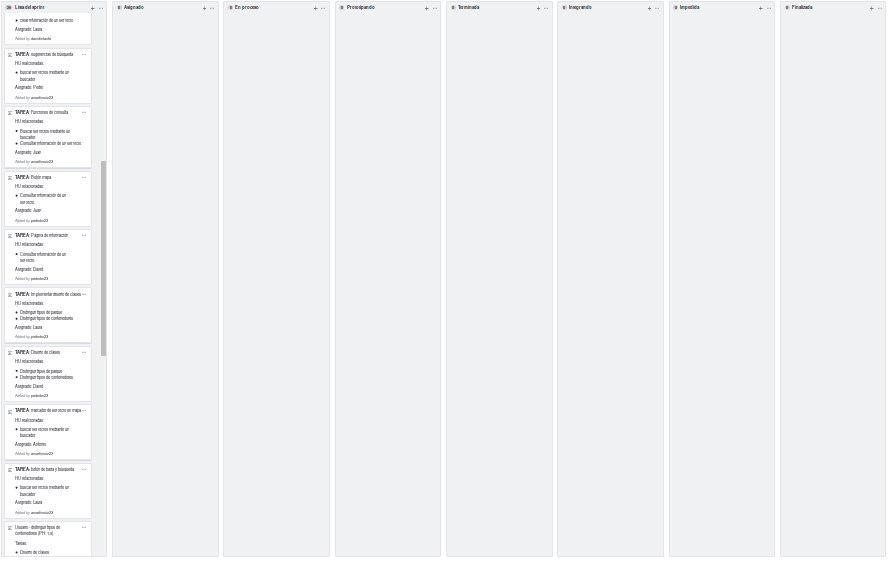
\includegraphics[width=\textwidth]{../imagenes/avance2-1.jpg}
\end{figure}

\end{frame}
\begin{frame}{Progreso Proyecto}

\begin{figure}
\centering
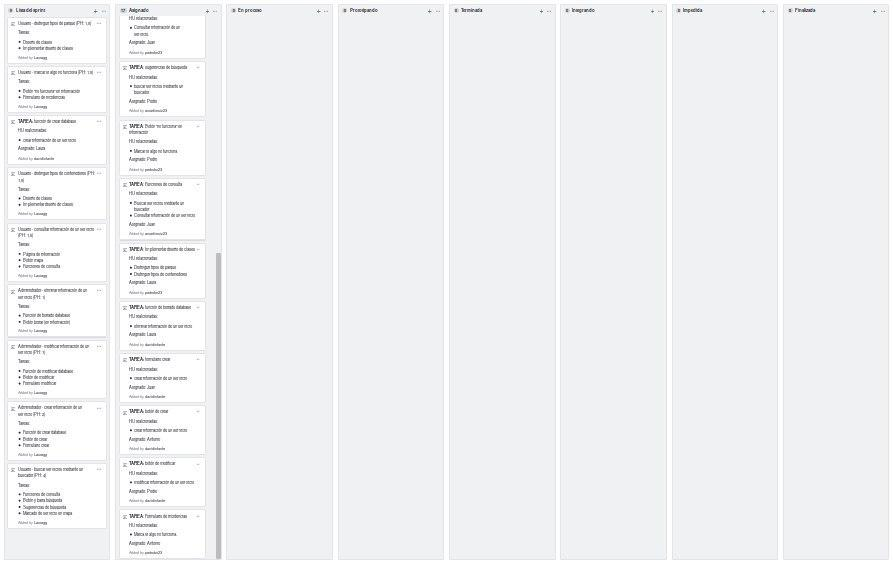
\includegraphics[width=\textwidth]{../imagenes/avance2-2.jpg}
\end{figure}

\end{frame}
\begin{frame}{Progreso Proyecto}

\begin{figure}
\centering
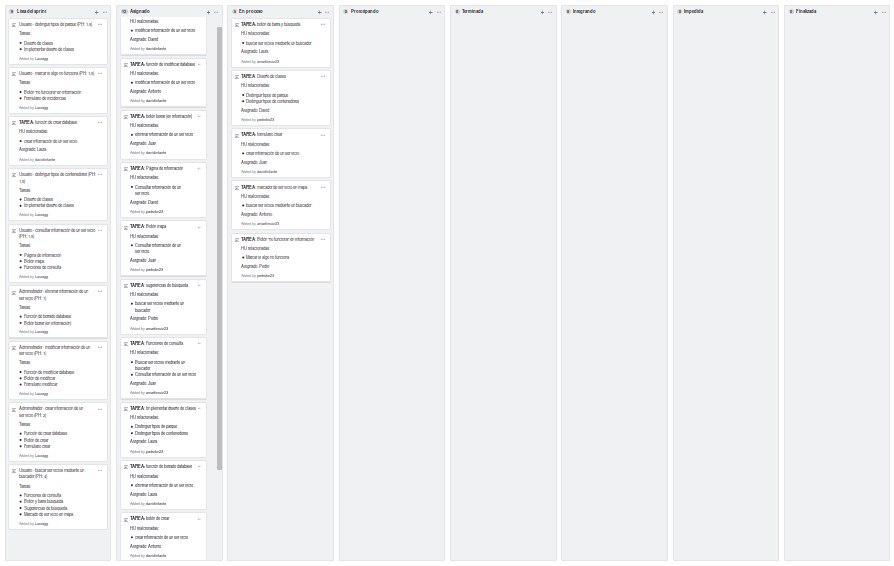
\includegraphics[width=\textwidth]{../imagenes/avance2-3.jpg}
\end{figure}

\end{frame}
\begin{frame}{Progreso Proyecto}

\begin{figure}
\centering
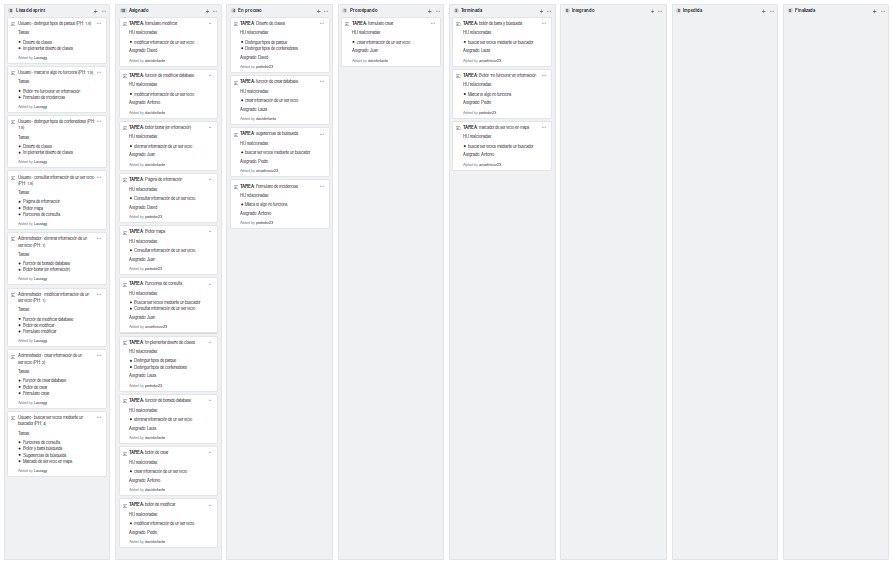
\includegraphics[width=\textwidth]{../imagenes/avance2-4.jpg}
\end{figure}

\end{frame}
\begin{frame}{Progreso Proyecto}

\begin{figure}
\centering
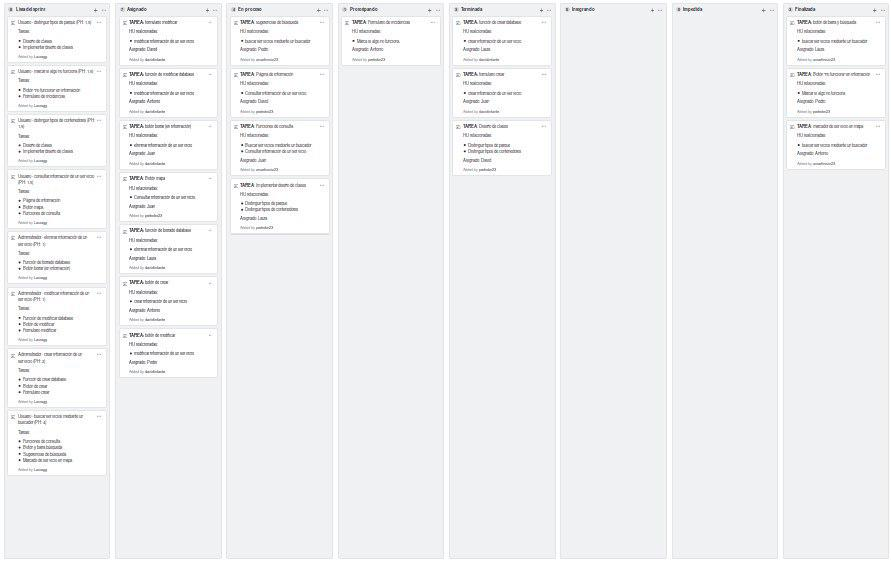
\includegraphics[width=\textwidth]{../imagenes/avance2-5.jpg}
\end{figure}

\end{frame}

\begin{frame}{Progreso Proyecto}

\begin{figure}
\centering
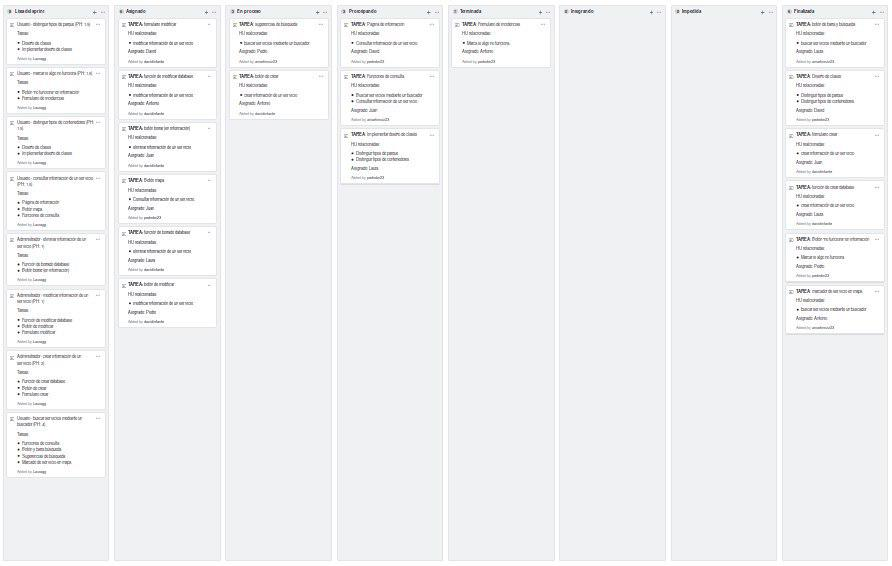
\includegraphics[width=\textwidth]{../imagenes/avance2-6.jpg}
\end{figure}

\end{frame}

\begin{frame}{Progreso Proyecto}

\begin{figure}
\centering
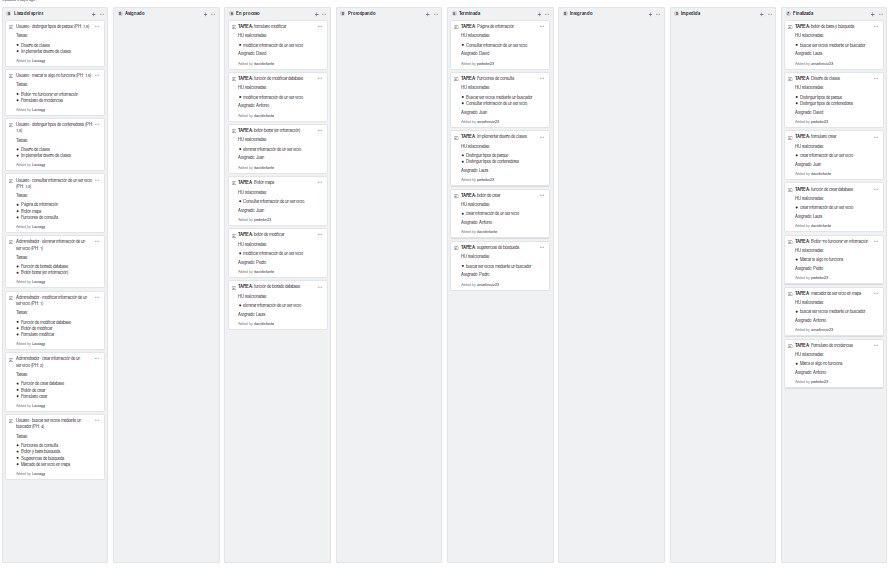
\includegraphics[width=\textwidth]{../imagenes/avance2-7.jpg}
\end{figure}

\end{frame}

\begin{frame}{Progreso Proyecto}

\begin{figure}
\centering
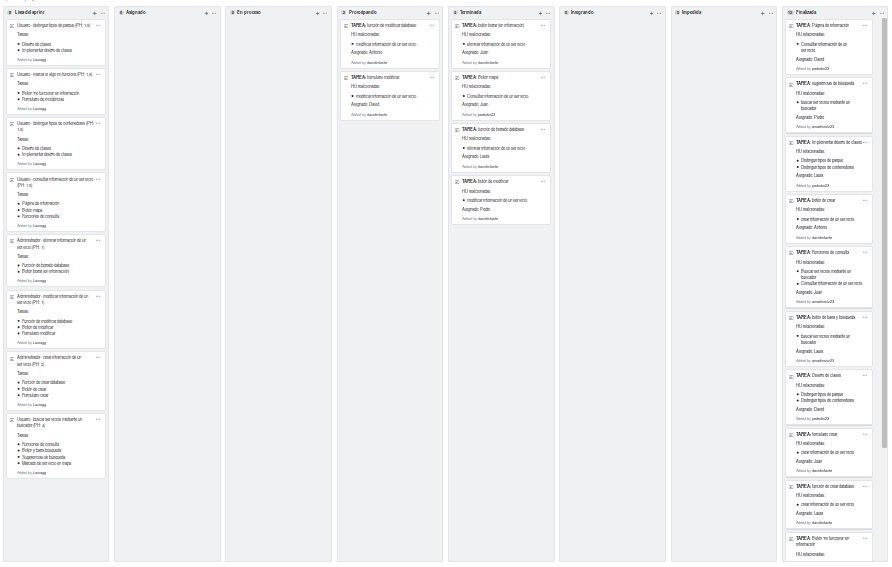
\includegraphics[width=\textwidth]{../imagenes/avance2-8.jpg}
\end{figure}

\end{frame}

\begin{frame}{Progreso Proyecto}

\begin{figure}
\centering
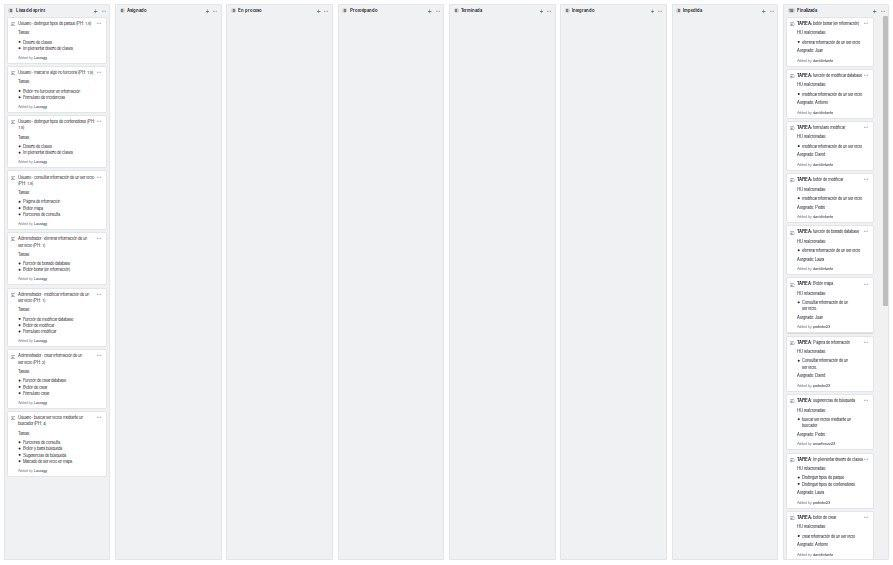
\includegraphics[width=\textwidth]{../imagenes/avance2-9.jpg}
\end{figure}

\end{frame}


\section{Prototipo}

\begin{frame}{Prototipo}

A continuación, una pequeña demo de nuestro prototipo.

\end{frame}

\end{document}